\documentclass[main.tex]{subfiles}

\begin{document}
\section{PCT Project}
\textit{This chapter covers the PCT-project that is currently under development at the Department of Physics and technology in Bergen. It discusses the DTC being developed for the project, how it tracks and measures the energy protons. Finally a technical overview of the system is given, along with how the Power Control System and the control software of this thesis will be implemented.}

The Bergen \gls{pct}-project is a collaboration with the University of Bergen and several other universities and institutions in the world. The purpose is to build a \gls{pct}-scanner to be used in proton treatment. The design is based on using a \acrlong{dtc} to detect protons emitted from the particle accelerator. In particular, the focus is on creating a scanner for use on pediatric patients.

\notinmain{start fra toppen av systemet, og så gå ned til sensorene}

\subsection{Introduction}

The \gls{pct}-project is comprised of several control systems and sensors. The main instrument is a \gls{dtc} that uses \gls{alpide}-chips to measure the energy of protons. The \gls{dtc} is made out of 43 layers of \gls{alpide} sensors and there are three control systems that oversee the \gls{dtc}. These systems are: cooling, readout, and power delivery. A simple schematic of the \gls{pct}-system is shown in \autoref{fig: pct_concept}.

\begin{figure}[!ht]
    \centering
    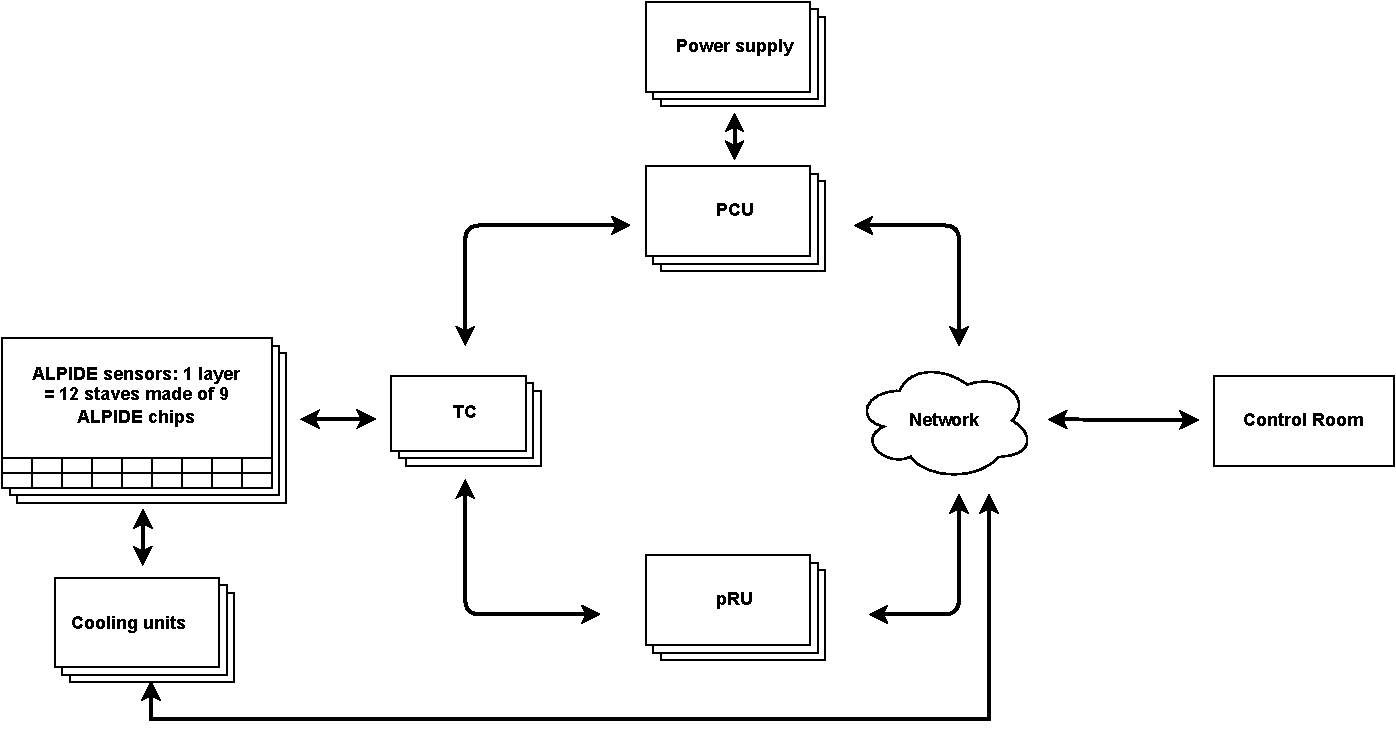
\includegraphics[width=15cm]{images/dcs_concept_renewed.pdf}
    \caption{Block diagram showing the general concept of the pCT System.}
    \label{fig: pct_concept}
\end{figure}
\FloatBarrier

The cooling system is obviously connected directly to the \gls{dtc}, while power delivery and readout perform their actions through a \gls{tc}. All systems is connected to a network that allows it to communicate with the Control Room, which is located on a computer.

The \gls{pct}-system is still under development, but \autoref{fig: pct_diagram} shows the current implementation of the system.

\begin{figure}[!ht]
    \centering
    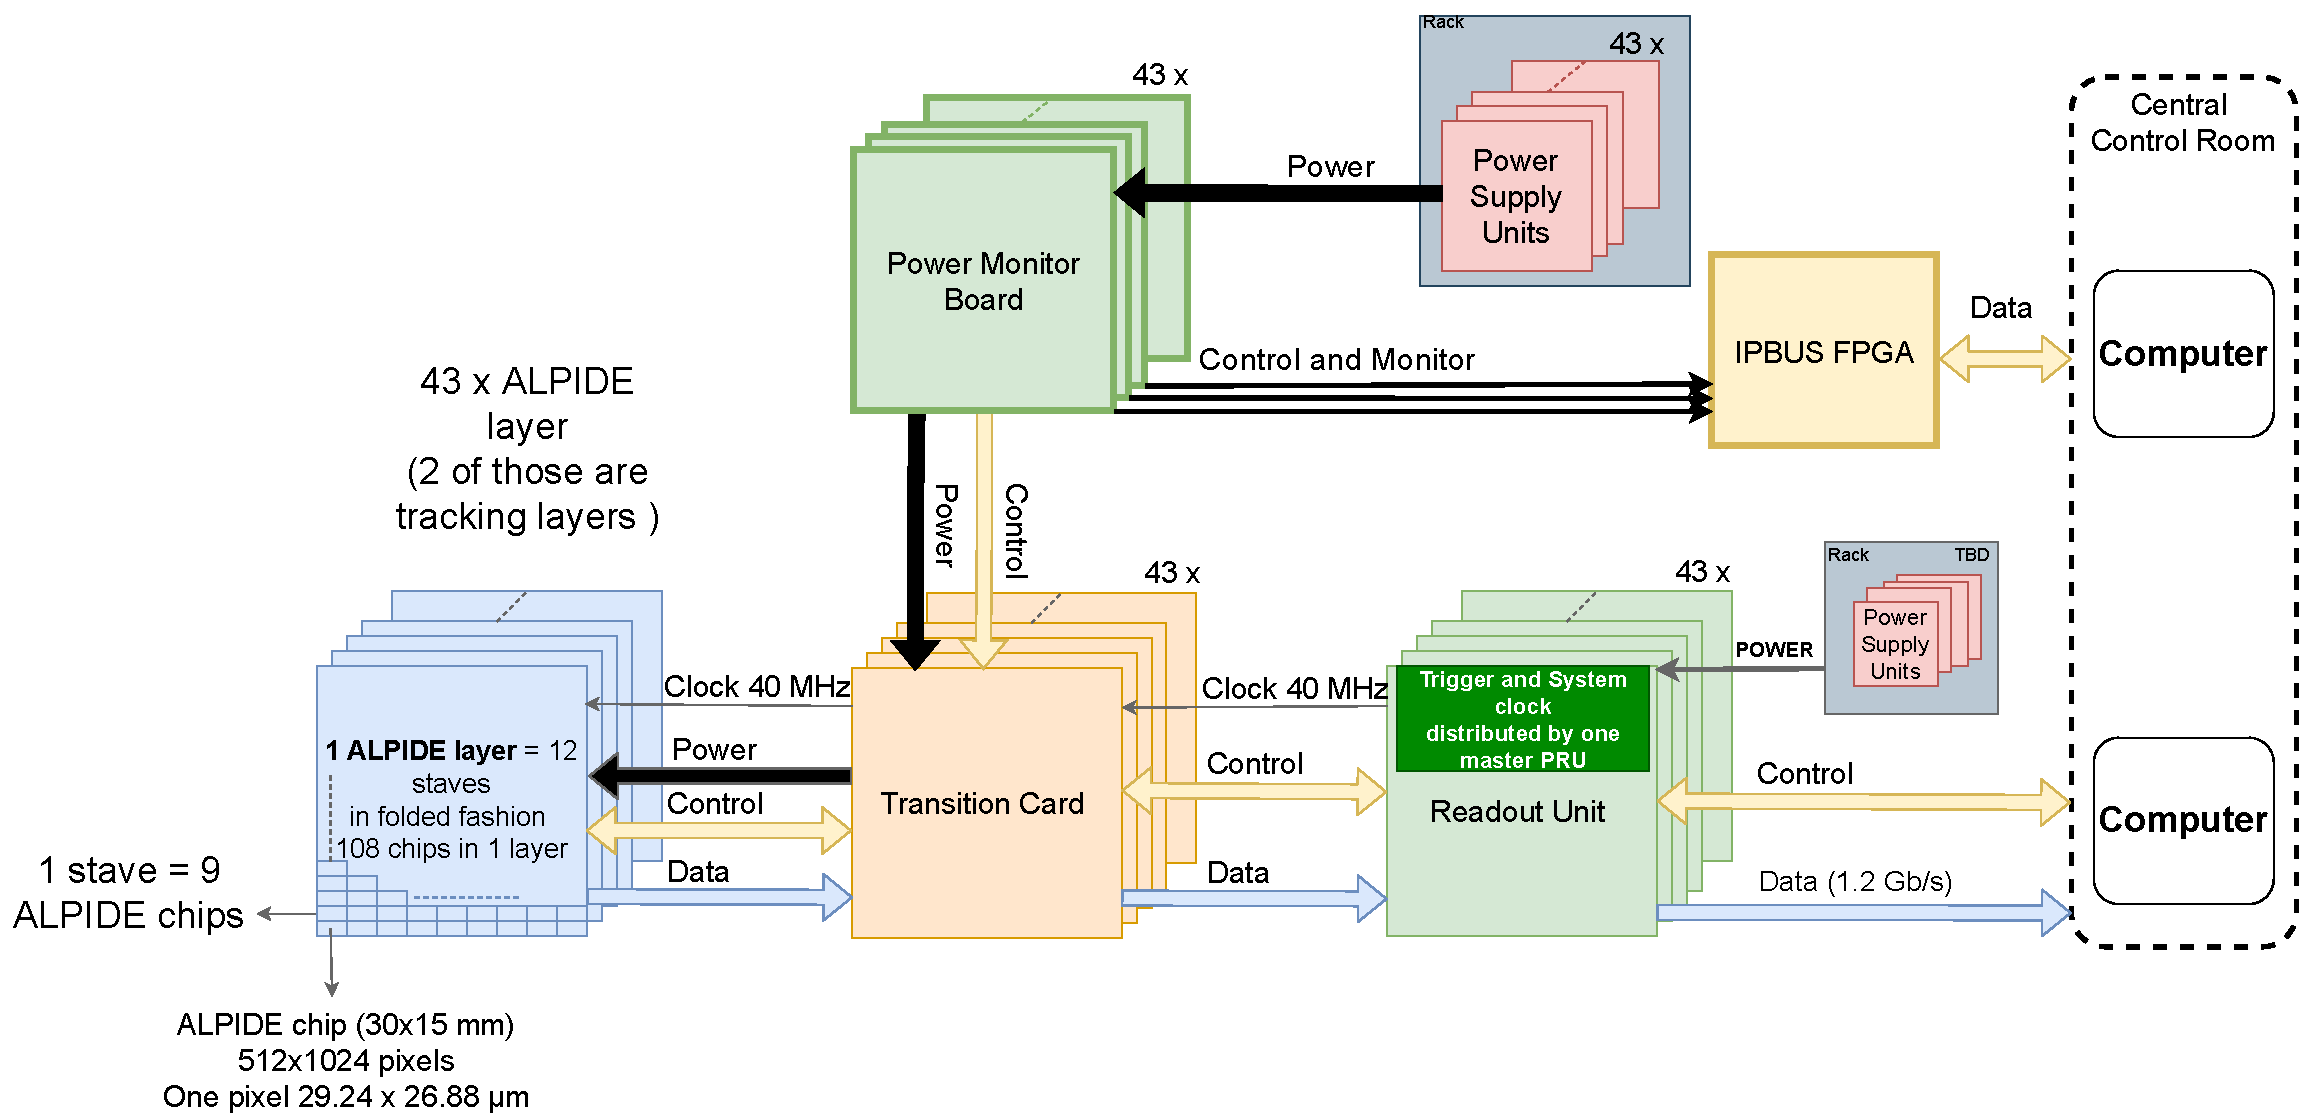
\includegraphics[scale=0.4]{images/pCT_Current_layout-CurrentSystemOverview.pdf}
    \caption{Block diagram of the current design of the pCT system. The upper part shows the power delivery and monitoring system, and lower half is the readout unit.}
    \label{fig: pct_diagram}
\end{figure}
\FloatBarrier


\subsection{DTC}

The \gls{dtc} is the main instrument of the \gls{pct}-system, it combines proton tracking and energy measurement into one technology. It is made out of 43 layers of pixel detectors, where 2 layers in the rear is used to track the trajectory of the protons and the other 41 measures their energy. A model of it is given in \autoref{fig: DTC_image}.

\begin{figure}[!ht]
    \centering
    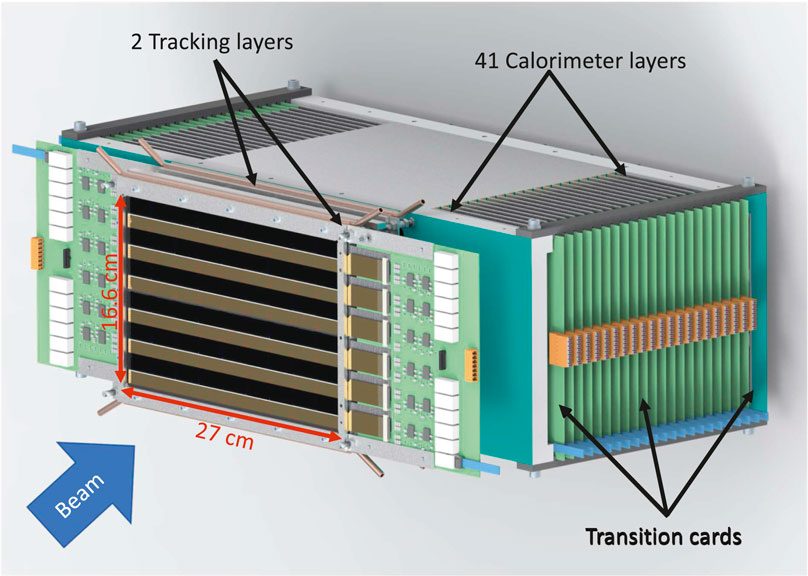
\includegraphics[scale = 0.5]{images/dtc.jpg}
    \caption{Model of DTC used in the pCT project. Dimensions of the tracker are (27 cm x 16.6 cm).}
    \label{fig: DTC_image}
\end{figure}
\FloatBarrier

A \gls{dtc} is usually realized with front and rear trackers, but only the rear trackers are used in this prototype. Studies have shown that single-sided proton imaging using Pencil Beam Scanning can lead to similar spatial resolution in the image as compared to double-sided\cite{pbs_result} imaging. the single-sided tracker also comes with a few advantages, such as lower material budget and less complexity in the rigging of the \gls{dtc}.

The layers of \gls{dtc} are functionally identical, but the calorimeter layers are made with aluminum absorbers to fully contain the energy range from the proton beam, which is estimated to be 230 MeV. The tracking layer must have minimum material budget to minimize the scattering of the protons, which can affect the accuracy of the image. The tracking layers are used to track the angle the protons exit the patient, the two layers provides the linear path of the proton and the angle is derived from that. Based on the angle, one can make an estimate of the most likely path taken by the protons as it was moving through the patient. This data is crucial for reconstructing the CT-image.

A layer of the \gls{dtc} is realized using 12 strings of \gls{alpide}-chips. a layer is made out of two half layers, and a half layer is made out of two "slabs of \gls{alpide}-chips. the "slabs" are three strings glued together, a picture of a half layer is shown in \autoref{fig: half_layer}.

\begin{figure}[!ht]
    \centering
    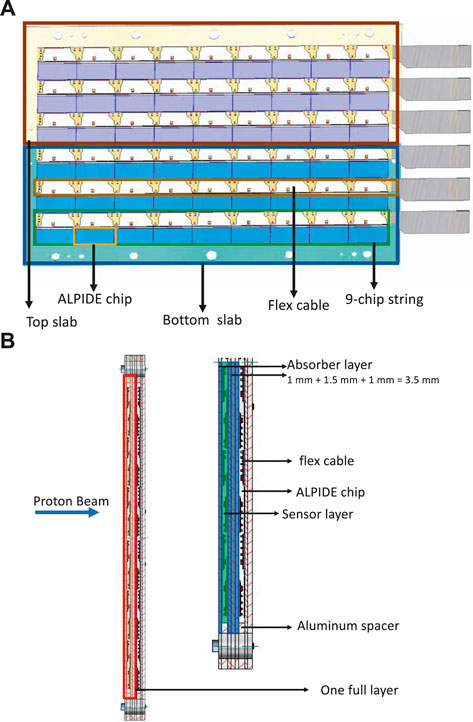
\includegraphics[scale = 0.5]{images/half_layer.jpg}
    \caption{A) Image of half layer, highlighting the various components of the layer. B) side view of a half layer and a full layer\cite{pct_project}}
    \label{fig: half_layer}
\end{figure}
\FloatBarrier

We can note from the figure that the \gls{alpide}-chip only covers about half of the layer, the rest of the space is dedicated to the flex cable. Two half layers are stacked in such a way that the \gls{alpide}-chips of one half layer covers the flex cable of the other, ensuring full area coverage. This gives us a full layer of the \gls{dtc}.


\subsection{ALPIDE chips}

The basic pixel detector sensor used for this project is the \gls{alpide}-chips that were designed for the upgrade of the \gls{its} during the long shutdown of the \gls{lhc} during the 2019-2020 period. The chips is categorized as \gls{maps} with a span of 1.5 cm x 3 cm. The sensor is made out of a matrix of 512 x 1024 pixels and they function as binary hit/no hit sensors. A detection threshold is set for the chip, suppressing all hits that are below the threshold level, functioning as data compression for non-relevant data, such as from noise and radiation. A cross section of the \gls{alpide} sillcon is shown in \autoref{fig: alpide_cross}.

\begin{figure}[!htpb]
    \centering
    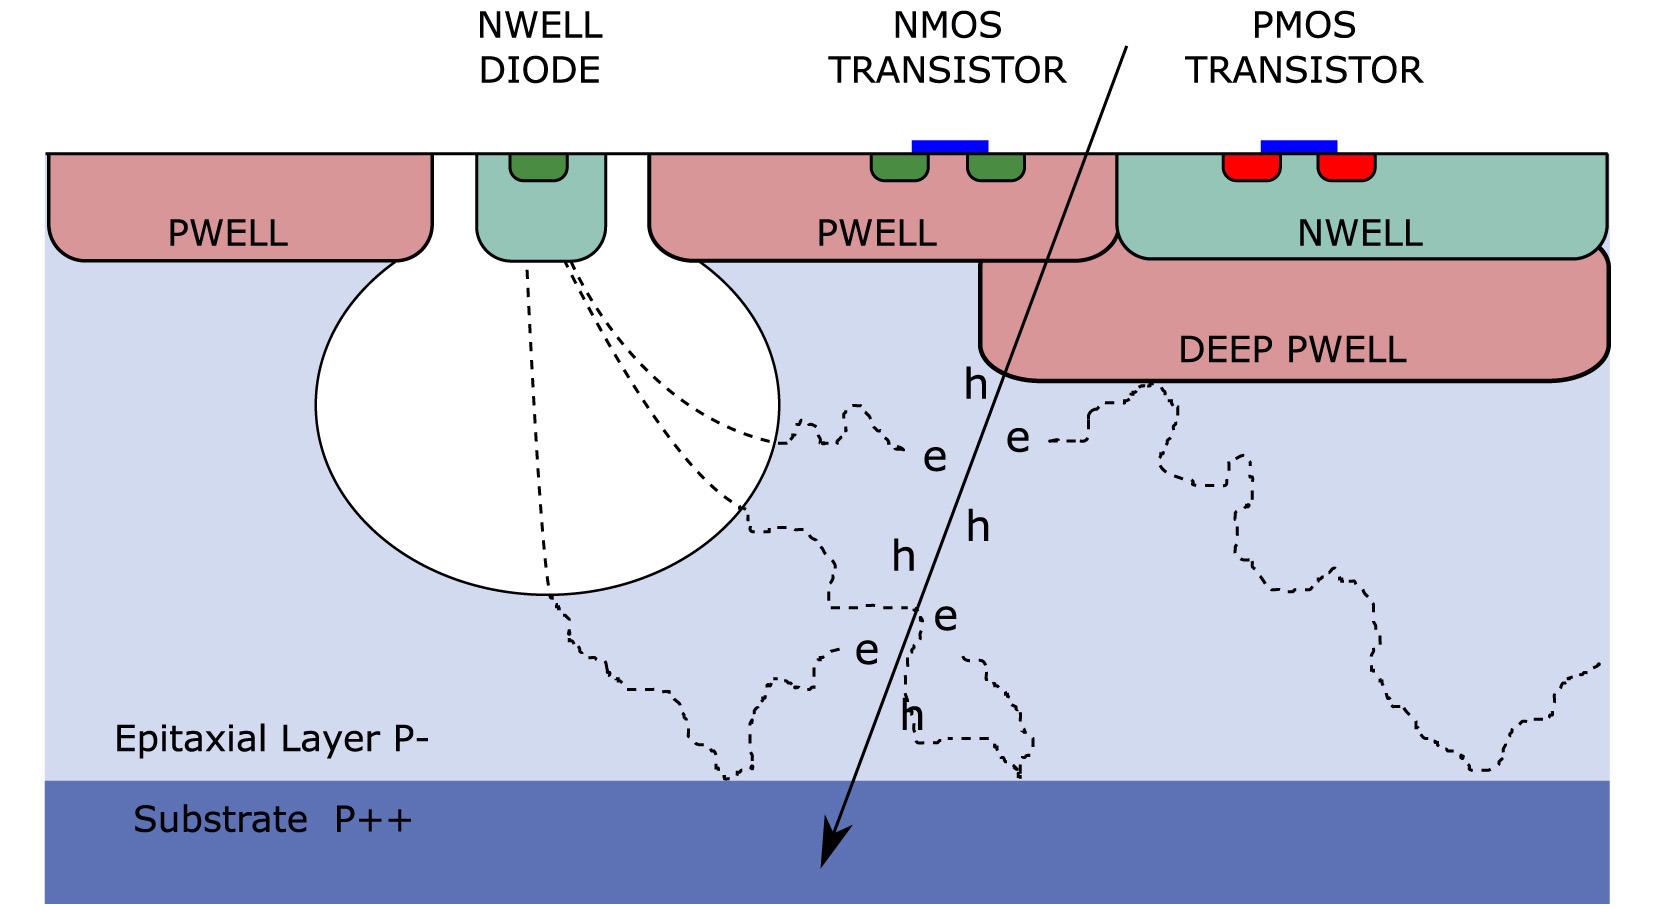
\includegraphics[width=12cm]{images/alpide_chip.jpg}
    \caption{Cross section of an ALPIDE-chip, showing a particle entering the silicon and causes a hit ot register.}
    \label{fig: alpide_cross}
\end{figure}
\FloatBarrier


The figure shows a particle entering the silicon and releasing electron-hole pairs from the Epitaxial layer. The charge moves to the depletion region around the collection diode and if it reaches the set threshold, registers a hit on the pixel.

In the \gls{pct} project, nine \gls{alpide}-chips are bonded together on one flex cable, which is defined as one "string". A \gls{alpide} string is shown in \autoref{fig: alpide_physical}.

\begin{figure}[!htpb]
    \centering
    \includegraphics[width=12cm]{images/alpideStringPhysical.png}
    \caption{Image of a string, highlighting the ALPIDE chip, chip cable, and flex cable.}
    \label{fig: alpide_physical}
\end{figure}
\FloatBarrier

From the figure we can see that half of the string is covered by the chip itself, and the other half is the flex cable the chips are mounted to.

For this thesis, it is also relevant to look at the power consumption of the strings. The \gls{alpide}-chips do not all draw the same amount of current, it is therefore necessary to measure the current draw of the strings. A test was performed on a string at UiB and it was recorded to draw 880 mA of digital current, and, a maximum analog current of 200 mA is also expected. Taking this into account, each string requires 1.9V and 1.1A to operate. 


\subsection{Cooling System}

The cooling system consists of two parts, one for the front tracking layers, and one for the calorimeter layers. The front tracking layers is cooled using liquid, while the calorimeter layers is cooled using five fans. Figure ?? shows the current implementation of the cooling system.

\notinmain{bilde av cooling system her}

The control of the cooling is done through maxz? cards, which is connected to the Control Room. The cooling system is monitored with four temperature sensors, two flow meters, and it can additionally monitor the RPM of the five fans. The control system for the cooling is still under development, currently it is only able to read out values from the sensors.


\subsection{Readout System}

The \gls{pct} readout system is comprised of 43 readout units, which acts as the communication hub between the Control Room and the sensors. Each layer has a corresponding \gls{pru}, which controls the sensors, as well as managing the data streams. The \gls{pru} board is realized using an Kintex Ultrascale KU085 \gls{fpga}, and the board is connected to the \gls{tc} using 12 Samtec FireFly cables. A block diagram of the board is shown in \autoref{fig: pru_diagram}.

\begin{figure}[!ht]
    \centering
    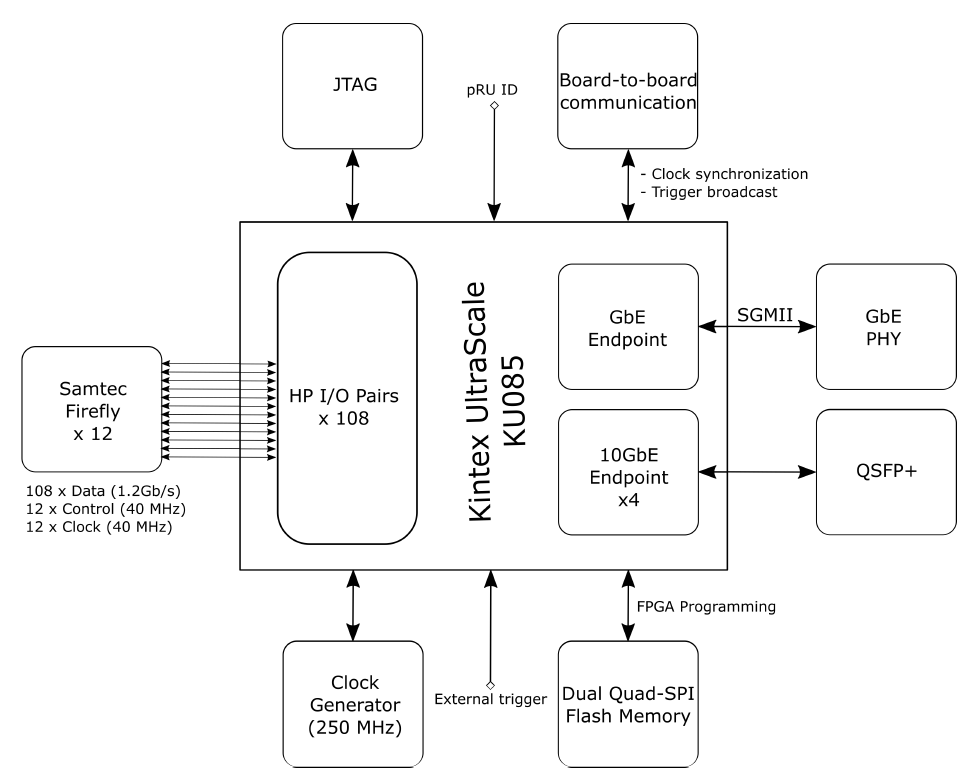
\includegraphics[scale=0.5]{images/pru_diagram.png}
    \caption{Simplified block diagram of the pRU board\cite{ola}}
    \label{fig: pru_diagram}
\end{figure}
\FloatBarrier

There is no monitoring system in place for the \gls{pru}, but a configuration system exists, which can store configuration values in a database and configure the strings. But this system is specialized, and will most likely require a new revision, to integrate with the rest of the \gls{pct}-system.

\subsection{Power Delivery System}

The power delivery system is responsible for powering the strings on the \gls{dtc}, and also monitor the performance of the strings. \autoref{fig: pds_diagram} outlines a detailed block diagram of the system.

\begin{figure}[!ht]
    \centering
    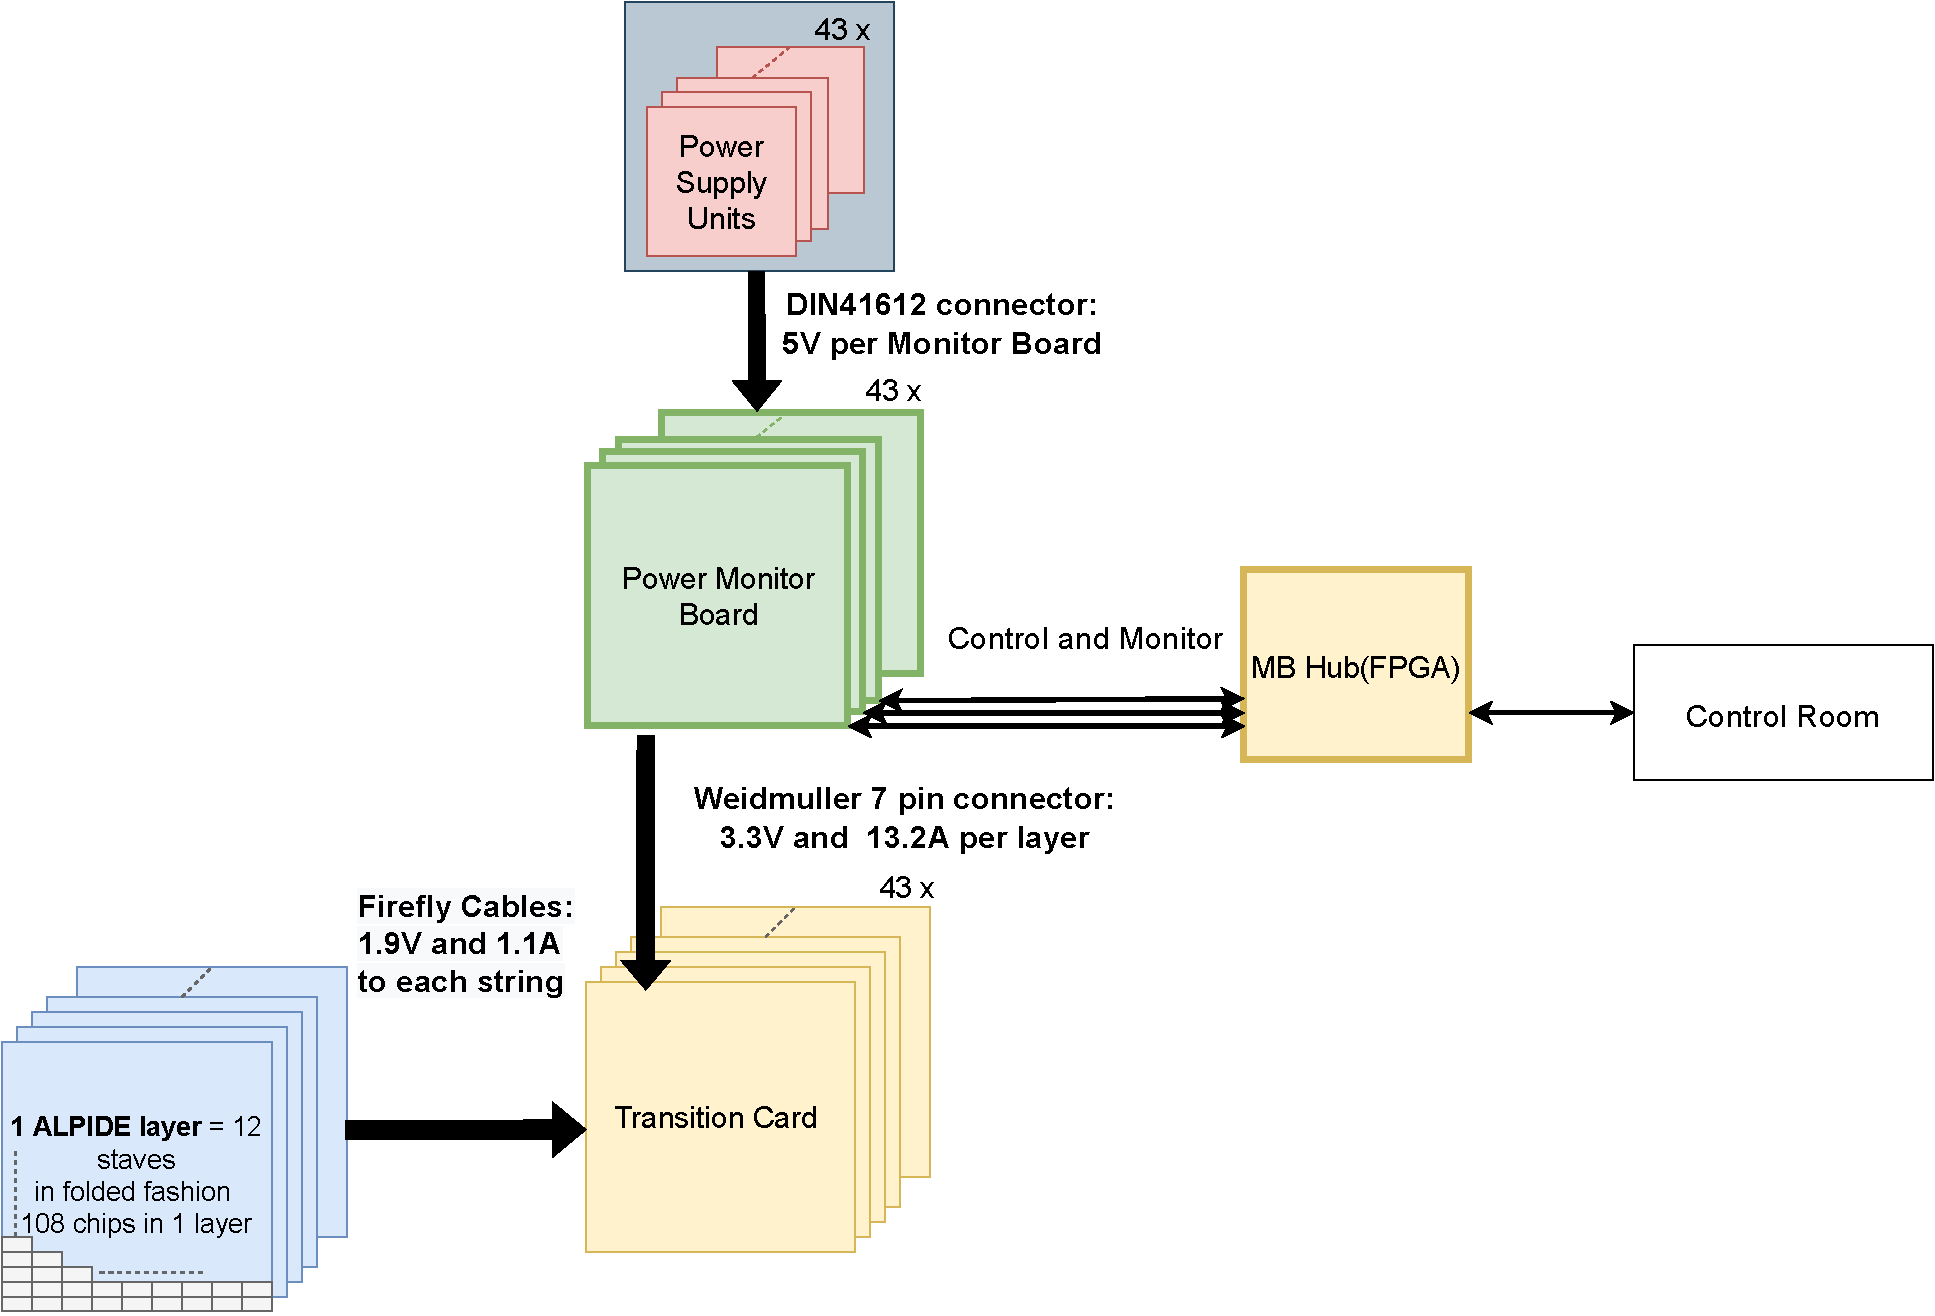
\includegraphics[scale=0.5]{images/pds_detail.pdf}
    \caption{Detailed block diagram of the power delivery system.}
    \label{fig: pds_diagram}
\end{figure}
\FloatBarrier

Control of the system is done through the Control Room, which uses the MB Hub to interface with the \acrlong{mb}s. The \gls{mb} delivers power from the PSU to the \gls{tc}. It also monitors the temperature and current usage of the strings. A string is turned off by the \acrlong{mb} if it exceeds the current/temperature threshold level. This ensures that the strings is turned off quickly, to not damage the chips. The \gls{mb}s deliver 3.3V to each \gls{tc}, which uses linear voltage regulators to shift the level down to 1.9V before delivering it to the strings.

The control system of the power delivery is discussed in \autoref{section: pcs}, where the focus is on the communication chain between the Control Room and the \acrlong{mb}s.

\notinmain{Vet ikke hvor denne skal gå: Another aspect to be considered in the \gls{dcs} is the radiation the various components are exposed to. The radiation from the proton therapy can have an adverse effect on circuitry and hardware. From \autoref{fig: dcs_diagram}, it is estimated that the \gls{tc} will be in the high radiation zone due to having to be close to the actual sensors, while the readout units and \gls{mb} will have minimal exposure to radiation, due to being separated by at least 3 metres of Firefly cables. Therefore it is not necessary to accommodate extra radiation protection for components involved in the power control and readout systems.}




\end{document}